\documentclass[times, utf8, diplomski]{fer}
\usepackage{booktabs}
\usepackage{breqn}
\usepackage{minted}
\usepackage{hyperref}
\usepackage{listings}
\usepackage{gensymb}
\usepackage{algorithm}
\usepackage{algpseudocode}
\usepackage[]{pdfpages}

\setminted{breaklines, framesep=2mm, fontsize=\footnotesize, numbersep=10pt, linenos}
\renewcommand\listingscaption{Kôd}

\makeatletter
\renewcommand{\ALG@name}{Algoritam}
\makeatother

% Expectation symbol
\DeclareMathOperator*{\E}{\mathbb{E}}

\begin{document}

% Broj rada
\thesisnumber{2857}

% Naslov rada
\title{Automatizirani razvoj agenata za različita okruženja}

% Autor rada
\author{Paulo Sanković}

\maketitle

% Ispis stranice s napomenom o umetanju izvornika rada. Uklonite naredbu \izvornik ako želite izbaciti tu stranicu.
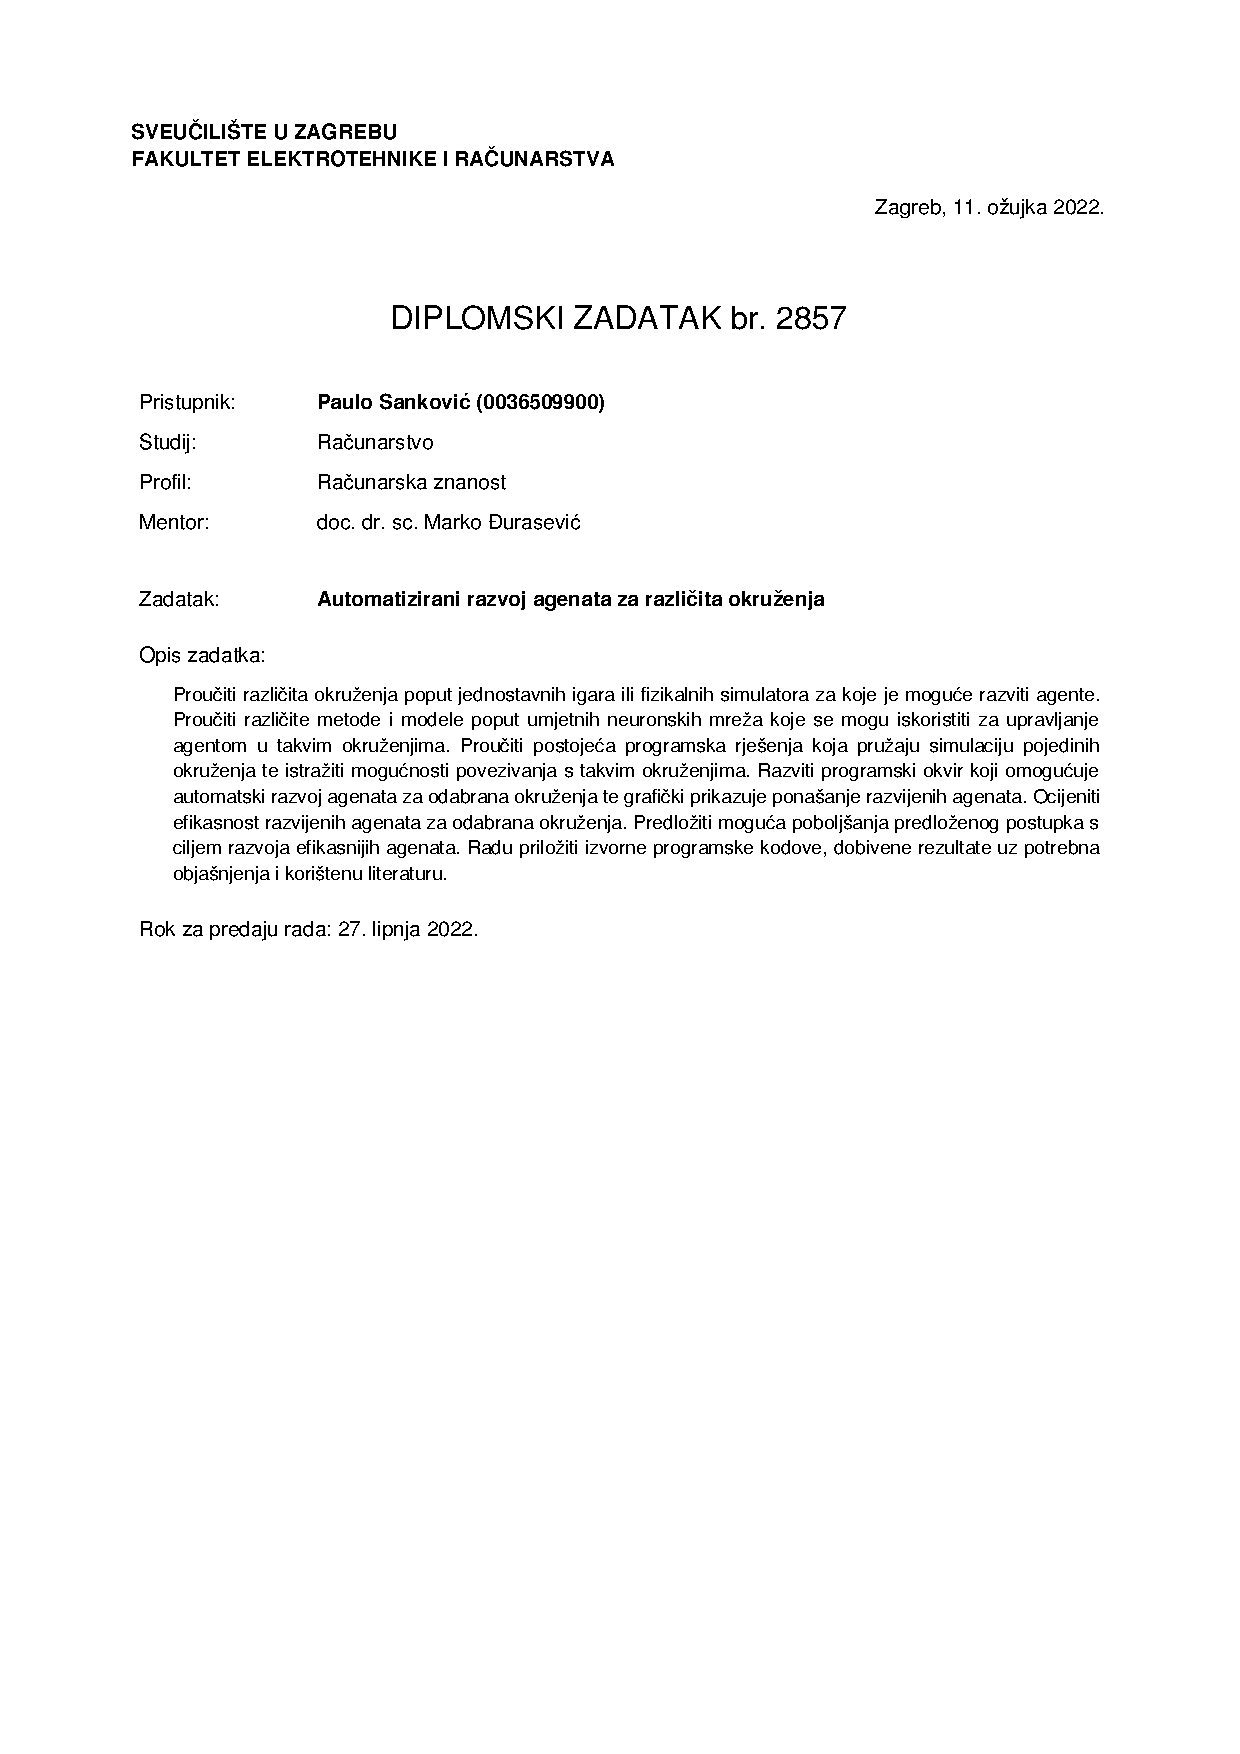
\includepdf[pages=-, noautoscale]{./assets/hr_0036509900_56.pdf}

% Dodavanje zahvale ili prazne stranice. Ako ne želite dodati zahvalu, naredbu ostavite radi prazne stranice.
\zahvala{Zahvaljujem se mentoru doc. dr. sc. Marku Đuraseviću na pomoći, dobrim savjetima i razumijevanju tijekom izrade ovog diplomskog rada, kao i svim profesorima i kolegama s kojima sam proveo svoje osnovnoškolske, srednjoškolske i studentske dane. Posebno bih se zahvalio svojoj obitelji na pruženoj podršci i razumijevanju.}

\tableofcontents

\chapter{Uvod}
Inteligentni sustavi sposobni su analizirati, razumjeti i učiti iz dostupnih podataka putem posebno dizajniranih algoritama umjetne inteligencije. Zahvaljujući dostupnosti velikih skupova podataka, razvoja tehnologije i napretka u algoritmima došli smo do razine gdje nam razvijeni modeli mogu uvelike poslužiti u svakodnevnom životu.

Posebno je zanimljiva problematika u kojoj je bez znanja o pravilima i funkcioniranju specifične okoline, potrebno konstruirati specijaliziranog agenta koji se nalazi u određenom stanju okoline i ponavlja korake izvršavanja optimalne akcije i prijelaza u novo stanje okoline. Za svaku akciju agent prima određenu nagradu - mjeru koja označava koliko su akcije agenta ispravne za tu okolinu i koliko je napredak agenta kvalitetan. Agent izvršava akcije i prelazi u nova stanja sve dok se ne nađe u terminalnom (završnom) stanju. Dakle, cilj agenta u okolini jest pronaći optimalnu strategiju koja će maksimizirati očekivanu dobit (nagradu) u određenom vremenskom okviru.

Područje strojnog učenja koje se bavi prethodno navedenom problematikom naziva se podržano učenje \engl{reinforcement learning}. Agenti koji se prilično dobro ponašaju u takvim okolinama možemo implementirati pomoću različitih algoritama podržanog učenja koji se temelje na umjetnim neuronskim mrežama \engl{artificial neural networks}. Umjetne neuronske mreže su dobri aproksimatori funkcija i najbolje se ponašaju u okolini koja ima kompozitnu strukturu gdje vrlo kvalitetno duboki model predstave kao slijed naučenih nelinearnih transformacija.

U sklopu ovog rada bilo je potrebno proučiti i razumjeti metode i algoritme podržanog učenja i funkcioniranje umjetnih neuronskih mreža. Nadalje, bilo je potrebno istražiti, proučiti i naposljetku implementirati neke od algoritama podržanog učenja koji se zasnivaju na umjetnim neuronskim mrežama i koje je trebalo uklopiti u okoline koje su prikladne za simulaciju i testiranje ponašanja naučenih agenta.

Programsko rješenje implementirano je u programskom jeziku \textit{Python}, primarno koristeći \textit{PyTorch} biblioteku \engl{library}, te ostale korisne biblioteke poput \textit{numpy}, \textit{tqdm}, \textit{stable-baselines3}, \textit{tensorboard}... Za simulaciju i testiranje ponašanja agenata u posebnom okruženju korištena je biblioteka \textit{OpenAI Gym}. 

\chapter{Podržano učenje}

Strojno učenje \engl{Machine learning} je grana umjetne inteligencije \engl{artificial inteligence} koje se može definirati kao skup metoda koje u podatcima mogu automatski otkrivati obrasce, i potom te otkrivene obrasce iskorištavati pri budućem predviđanju podataka, ili obavljati druge zadatke odlučivanja u prisustvu nesigurnosti \cite{CupicUvod}. Drugim riječima, bez eksplicitnog programiranja moguće je napraviti sustave koji funkcioniraju kao ljudski mozak - imaju pristup podatcima, koriste ih za učenje i samim time bolje razumiju entitete, domene i veze između podataka. 

Strojno učenje dijeli se na 3 podvrste: nadzirano učenje, nenadzirano učenje i podržano (ojačano) učenje. Nadzirano učenje \engl{supervised learning} karakterizira učenje modela nad testnim podatcima koji su označeni. Model točno zna da za određeni ulaz mora vratiti izlaz koji je istovjetan unaprijed pridruženoj oznaci. Algoritam mjeri točnost kroz funkciju gubitka, prilagođavajući se sve dok se izračunata razlika izlaza modela i stvarnog izlaza (pogreška) ne smanji do određene mjere. S druge strane, u nenadziranom učenju \engl{unsupervised learning} posjedujemo podatke bez zadanog izlaza - podatci su dani bez ciljne vrijednosti i u tim situacijama treba pronaći određenu pravilnost. Postupci poput grupiranja, smanjenja dimenzionalnosti, otkrivanja veza između primjeraka... pripadaju nenadziranom učenju.

Posebna i nama najzanimljivija podvrsta strojnog učenja jest podržano učenje (engl. \textit{reinforcement learning}). Podržano učenje bavi se optimizacijom ponašanja agenta koji je u interakciji s okolinom (u kojoj se nalazi) i koji izvršava akcije na temelju informacija koje dobiva iz okoline. Agent pri svakom koraku od okoline dobiva povratnu informaciju u obliku nagrade ili kazne. Za razliku od prethodne dvije navedene podvrste koje mapiraju ulazne podatke na određeni format izlaza, u podržanom učenju je najizraženije učenje iz iskustva koje je čovjeku i drugim živim bićima veoma blisko.

\section{Ključni koncepti}

Za potpuno razumijevanje podržanog učenja, bitno je u navesti i pojasniti ključne koncepte i terminologiju. Okolina \engl{environment} označava svijet u kojem se agent nalazi i s kojim interaktira. Stanje $s_t$ \engl{state} reprezentira kompletni opis okoline u određenom trenutku $t$. S druge strane, opservacija okoline $o_t$ \engl{observation} predstavlja prilagođeni i ograničeni opis okoline koji agent dobije u nekom trenutku. Kada se agent nađe u nekom stanju $s_t$ i kada od okoline dobije opservaciju $o_t$, tada agent poduzima akciju $a_t$ \engl{action} i samim time u idućem vremenskom koraku inicira promjenu stanja $s_{t+1}$ i opservacije okoline $o_{t+1}$. 

Način na koji agent odabire akciju iz skupa svih dostupnih akcija naziva se politika \engl{policy}. Politika ovisi o parametrima modela $\theta$ i može biti deterministička $\mu_{\theta}$ ili stohastička $\pi_{\theta}$. Veza između akcije, politike i stanja prikazana je izrazima \ref{md:policy}. U našem slučaju koristiti ćemo politike koji su zapravo duboki modeli - aproksimacije funkcije odluke čiji se parametri uče optimizacijskim algoritmima.  

\begin{equation}
    \begin{gathered}
    \label{md:policy}
    a_t = \mu_{\theta}(s_t) \\
    a_t \sim \pi_{\theta}(\cdot \mid s_t)
    \end{gathered}
\end{equation}

Nadalje, putanja $\tau$ \engl{trajectory} je pojam koji označava niz stanja i pripadajućih akcija i predstavljen je izrazom \ref{md:trajectory}. Interakcija s okolinom započinje u trenutku $t = 0$ kada pomoću funkcije za inicijalizaciju okoline $\rho_0$ poštujući pravila okoline, nasumično generiramo stanje $s_0$.

\begin{equation}
    \label{md:trajectory}
    \tau = (s_0, a_0, s_1, a_1, ...)
\end{equation}

Najvažnija i najkorisnija informacija koju agent dobiva od okoline jest nagrada $r_t$ \engl{reward} koju generira funkcija $R$ \engl{reward function} i koja u obzir uzima trenutno i iduće stanje te akciju koja je izazvala promjenu stanja. Povezanost između generiranja iznosa nagrade i same nagrade prikazana je izrazom \ref{md:reward}.

\begin{equation}
    \label{md:reward}
    r_t = R(s_t, a_t, s_{t+1})
\end{equation}

Želimo dobiti što bolji pregled koliko su bile dobre akcije koje je agent poduzeo. Tu informaciju možemo predstaviti na dva različita načina. Sumom nekorigiranih nagrada zbrajamo samo nagrade koje su dobivene u fiksnom vremenskom intervalu $T$ (izraz \ref{md:undiscounted-return}). Na taj način dobivamo informaciju o tome kolika je bila prosječna nagrada u zadnjih $T$ koraka. Ako pak želimo pokazati da su nam nagrade u trenutnom stanju vrjednije nego nagrade koje ćemo dobiti u budućim stanjima, moramo uvesti korekcijski faktor $\gamma \in (0,1)$ \engl{discount factor}. Navedeni pristup sumiranja korigiranih nagrada prikazan je izrazom \ref{md:discounted-return}.

\begin{equation}
    \label{md:undiscounted-return}
    R(\tau) = r_0 + r_1 + ... + r_T = \sum_{t=0}^{T}r_t
\end{equation}

\begin{equation}
    \label{md:discounted-return}
    R(\tau) = r_0 + \gamma \cdot r_1 + \gamma^2 \cdot t_2 + \gamma^3 \cdot t_3 + ... = \sum_{t=0}^{\infty}\gamma^t r_t
\end{equation}

% TODO na sve ovo dodati literaturu https://spinningup.openai.com/en/latest/spinningup/rl_intro.html i http://java.zemris.fer.hr/nastava/ui/rl/rl-20200401.pdf

Dakle, cilj podržanog učenja jest naći optimalnu strategiju (niz optimalnih akcija) koje maksimiziraju ukupnu (kumulativnu) nagradu. U svakom koraku interakcije agenta s okolinom, agent prima opis stanja okoline u kojoj se nalazi. S obzirom na to stanje, izvršava akciju koja vrši neku promjenu nad okolinom i prebacuje ju u novo stanje. Agent prima povratnu informaciju od okoline koja reprezentira koliko je odabrana akcija dobra. Opisana interakcija agenta i okoline prikazana je na slici \ref{fig:rl}.

\begin{figure}[H]
    \centering
    \frame{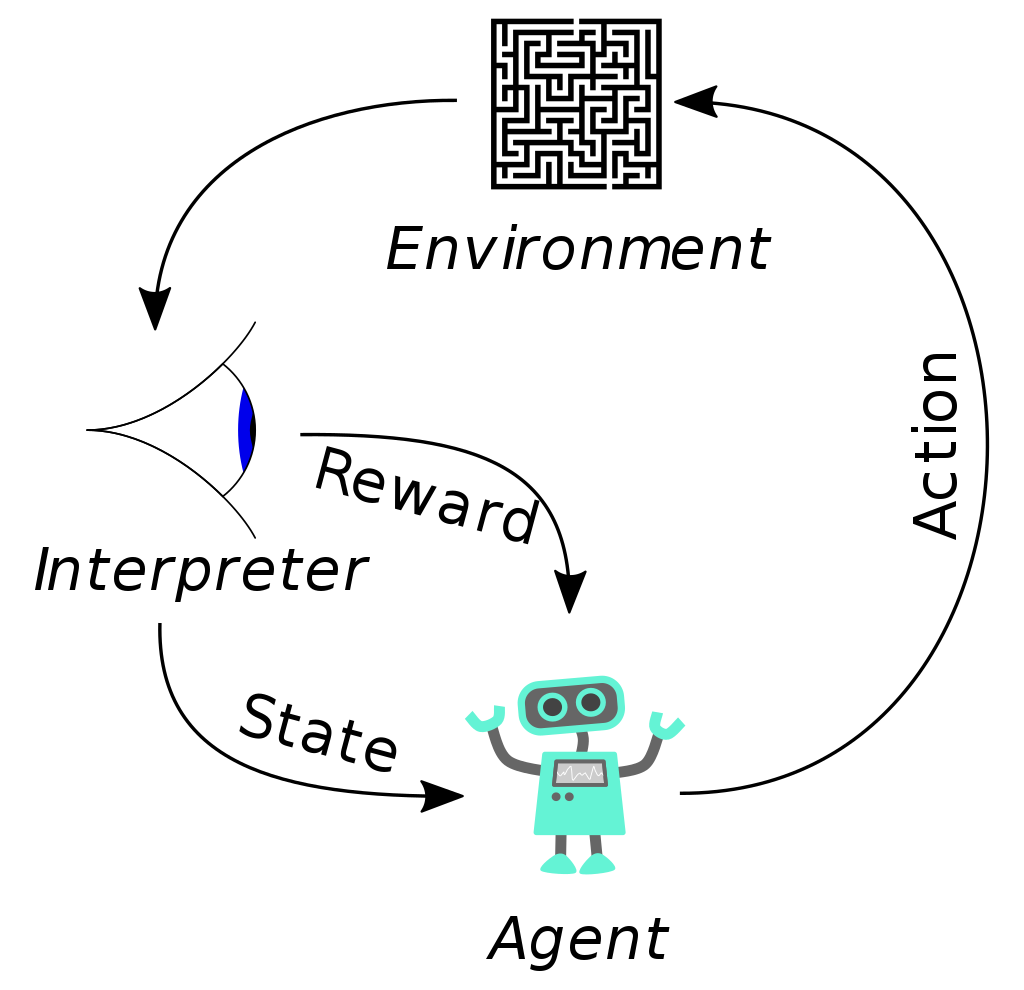
\includegraphics[width=7cm]{assets/rl_diagram.png}}
    \caption{Ciklus interakcije agenta s okolinom - TODO ref}
    \label{fig:rl}
\end{figure}

\section{Duboki modeli}

Duboko učenje \engl{Deep learning} jest tip strojnog učenja (točnije, podskup strojnog učenja) koje nastoji oponašati način zaključivanja i obrasce koje ljudski mozak koristi za učenje i donošenje odluka. Veliku ulogu u cijeloj ideji dubokog učenja imaju duboke neuronske mreže \engl{deep neural networks, DNN} pomoću kojih se povezivanjem više slojeva procesnih elemenata (čvorova, neurona), dobivaju duboki modeli koji su sposobni učiti i baratati s podatcima kompozitne strukture. Primjenom dubokih modela dolazimo do slijeda naučenih nelinearnih transformacija kojima aproksimiramo funkciju odluke, učimo mapiranje između ulaznih podataka i izlazih podataka, te nastojimo postići dobru generalizaciju nad stvarnim podatcima. 

\subsection{Unaprijedni potpuno povezani modeli}

Unaprijedni potpuno povezani modeli \engl{Fully connected neural network} (poznatiji i pod nazivom višeslojni perceptron \engl{Multi-layer perceptron}) sastoje se od lanaca potpuno povezanih slojeva. Svaki neuron iz prethodnog sloja povezan je s neuronom idućeg sloja. 

Sastoje se od tri vrste slojeva - ulaznog sloja, izlaznog sloja i skrivenih slojeva. Ulaznom sloju dovode se podatci koje je potrebno obraditi. Izlaz neuronske mreže (u najosnovnijem obliku) predstavljen je logitima \engl{logits} - vektorima logaritama nenormaliziranih vrijednosti. Specifičnije, za slučaj da želimo provesti klasifikaciju podataka ili drugačije organizirati izlazne vrijednosti na izlaz dodajemo posebni sloj (npr. \textit{Softmax} funkcija za klasifikaciju). Samo su ulaz i izlaz specificirani dimenzijama. Model ima slobodu da iskoristi skrivene slojeve na način koji osigurava najbolju aproksimaciju funkcije. Neuronskim mrežama želimo izgraditi modele koji nisu linearno odvojivi i zato koristimo nelinearnu aktivacijsku funkciju - najčešće ReLU (Rectified Linear Unit). Svaki od slojeva modelira jednu nelinearnu transformaciju.

Slika \ref{fig:nn} \cite{NNsvg} prikazuje arhitekturu potpuno povezanog modela koji je sastavljen od sveukupno 4 potpuno povezana sloja - ulaznog (dimenzije 4), izlaznog (dimenzije 2) i dva skrivena sloja (svaki dimenzije 8). Kodom \ref{lst:fcn} prikazana je implementacija navedenog modela u biblioteci \textit{PyTorch}.

\begin{figure}[H]
    \centering
    \frame{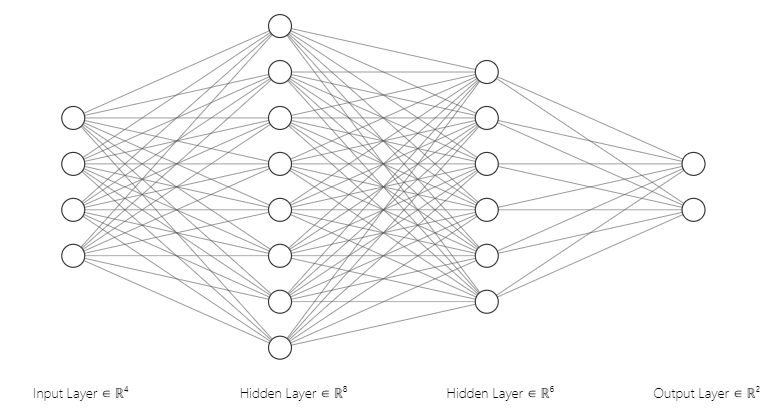
\includegraphics[width=11cm]{assets/nn.png}}
    \caption{Arhitektura potpuno povezanog modela}
    \label{fig:nn}
\end{figure}

\begin{listing}[H]
    \caption{Implementacija potpuno povezanog modela na slici \ref{fig:nn} koristeći biblioteku \textit{PyTorch}}
    \inputminted{python}{snippets/fcn.py}
    \label{lst:fcn}
\end{listing}

\subsection{Konvolucijski modeli}

Konvolucijski modeli \engl{Convolutional neural networks} su modeli koji uz potpuno povezane slojeve imaju najmanje jedan konvolucijski sloj \engl{convolution layer}. Osim spomenutih slojeva, konvolucijski modeli sadrže i slojeve sažimanja \engl{pooling layers}, slojeve u kojima provodimo nelinearnost podataka te sloj koji višedimenzionalni ulaz pretvara u jednodimenzionalni i pritom priprema podatke za obradu u potpuno povezanim slojevima \engl{flatten layer}.

Operacija konvolucije provodi se nad ulazom i jezgrom \engl{kernel} (slobodnim parametrima koje učimo) gdje kao rezultat dobivamo mapu značajki koja pokazuje gdje se koja značajka nalazi u ulaznim podatcima (npr. slici). Dimenzije mapa značajki i njihovu robusnost korigiramo korištenjem atributa koraka konvolucije \engl{stride} i nadopunjavanja ulaznih podataka \engl{padding}. Slično konvolucijskom sloju, sloj sažimanja odgovoran je za smanjenje prostora značajki (smanjenje dimenzionalnosti podataka) i dodatno za izdvajanje dominantnih značajki. Razlikujemo dvije vrste sažimanja: sažimanje maksimalnom vrijednosti \engl{max pooling} i sažimanje srednjom vrijednosti \engl{average pooling}. Prilikom sažimanja značajki maksimalnom vrijednošću u obzir uzimamo samo značajku najveće vrijednosti te na taj način uklanjamo šum ulaza i potencijalno biramo značajku najveće važnosti.

Korištenje konvolucijskih modela biti će nam iznimno potrebno u situacijama kada su ulazni podatci u formi slike, odnosno kada su nam važne lokalne interakcije između ulaznih podataka (piksela) te njihova vremenska i prostorna ovisnost.

Slika \ref{fig:cnn} \cite{NNsvg} prikazuje jednostavni konvolucijski model koji se sastoji od konvolucijskog sloja, sloja sažimanja maksimalnom vrijednosti, sloja koji $3$-dimenzionalne podatke pretvara u $1$-dimenzionalne, te dva potpuno povezana sloja. Ulaz u konvolucijski sloj predstavlja RGB slika (3 kanala) dimenzije $32 \times 32$. Primjenom konvolucije (veličina jezgre 3, korak 3, nadopuna 1) izvlačimo 18 kanala značajki dimenzije $32 \times 32$ (dimenzija se nije promijenila iz razloga što nadopunjavamo ulaz). Primjenom sažimanja maksimumom (veličina jezgre 2, korak 2) smanjujemo broj značajki na dimenziju $16 \times 16$. Prvi potpuno povezani sloj na svoj ulaz dobije vektor dimenzije $4608$ kojeg pretvara u vektor izlaza dimenzije $64$. Posljednji potpuno povezani sloj koji je ujedno i posljednji sloj u ovom konvolucijskom modelu za izlaz predaje vektor dimenzije $10$. Isječak koda koji prikazuje implementaciju jednostavnog konvolucijskog modela koristeći bibilioteku \textit{PyTorch} prikazan je kodom \ref{lst:cnn}.

\begin{figure}[H]
    \centering
    \frame{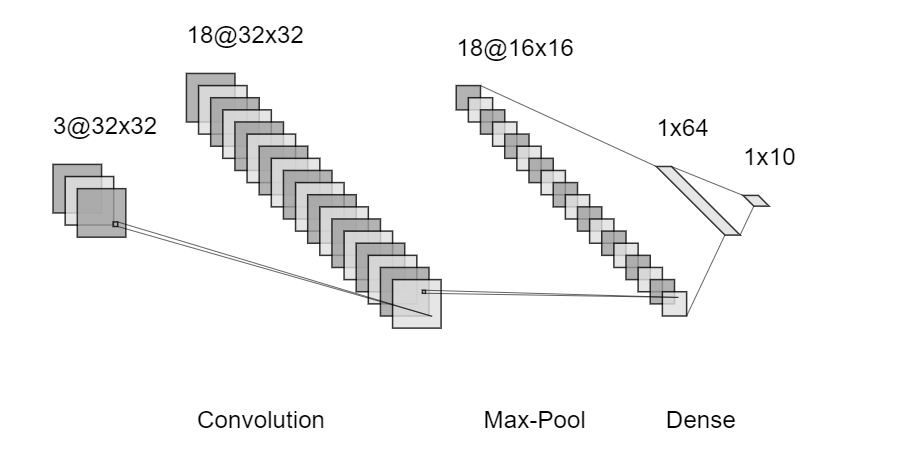
\includegraphics[width=11cm]{assets/cnn.png}}
    \caption{Arhitektura konvolucijskog modela}
    \label{fig:cnn}
\end{figure}

\begin{listing}[H]
    \caption{Implementacija konvolucijskog modela na slici \ref{fig:cnn} koristeći biblioteku \textit{PyTorch}}
    \inputminted{python}{snippets/cnn.py}
    \label{lst:cnn}
\end{listing}

\section{Algoritmi podržanog učenja}

Svaki algoritam strojnog učenja definiran modelom, gubitkom i metodom optimizacije. Model je postupak obrade (odnosno skup funkcija) sa slobodnim parametrima koji za određen ulaz daje pripadajući izlaz. Gubitak je mjera koja na formaliziran način vrednuje slobodne parametre modela, odnosno pokazuje u kojoj mjeri se mi ne slažemo s onim što je model predstavio kao izlaz. Metoda optimizacije (optimizacijski postupak) jest način na koji pronalazimo optimalne parametre koji su važni kako bi minimizirali prethodno navedenu komponentu - gubitak. Navedene tri glavne komponente biti će važno napomenuti pri svakom predstavljaju algoritma jer su to glavne odrednice pri analizi algoritama strojnog učenja.

TODO dodati dio oko value functions, advantage functions... kako bi bilo kasnije lakše objasniti algoritme, funkcije gubitka, što koja mreža predstavlja...

% https://spinningup.openai.com/en/latest/spinningup/rl_intro2.html

% dodati literaturu https://www.fer.unizg.hr/_download/repository/SU-2020-02-OsnovniKoncepti.pdf

\subsection{Deep Q Learning}

TODO https://github.com/udacity/deep-learning/blob/master/reinforcement/nature14236.pdf

\subsection{Double Deep Q Learning}

TODO https://arxiv.org/pdf/1509.06461.pdf

\subsection{Actor Critic}

TODO https://www.tensorflow.org/tutorials/reinforcement_learning/actor_critic

\chapter{OpenAI Gym}

OpenAI Gym je Python biblioteka \engl{library} otvorenog koda \engl{open source} koja služi za razvijanje i usporedbu agenata u odabranim okolinama. Iznimno je popularna u sferi simpatizera i programera koji se bave razvijanjem modela podržanog učenja zbog jednostavnosti korištenja, velikog broja dostupnih okolina i jednostavnog stvaranja novih okolina, te jednostavne interakcije agenta i okoline. OpenAI Gym biblioteka se redovito održava i trenutno je na verziji \texttt{0.24.1}. 

\section{Struktura}

Interakcija agenta i okoline podijeljena je na epizode. Na početku svake epizode, početno stanje se nasumično uzorkuje iz distribucije, i interakcija se nastavlja sve dok se okolina ne nađe u terminalnom stanju \cite{OpenAIWhitepaper}.

\begin{listing}[H]
    \caption{Jednostavan primjer integracije agenta i Gym okoline (1 epizoda)}
    \inputminted{python}{snippets/init.py}
    \label{lst:init-code}
\end{listing}

Kod \ref{lst:init-code} prikazuje potpunu implementaciju jednostavne interakcije agenta i okoline. Agent u ovom jednostavnom slučaju nasumično odabere akciju iz skupa svih dostupnih akcija za tu okolinu (linija 9). Osnovni kostur sastoji se od koraka specifikacije okoline (linija 3), inicijalizacije okoline (linija 5) te interakcija okoline i agenta - agent predaje okolini odabranu akciju, okolina vraća povratnu informaciju (linije 7 - 14). 

\begin{figure}[h]
    \centering
    \frame{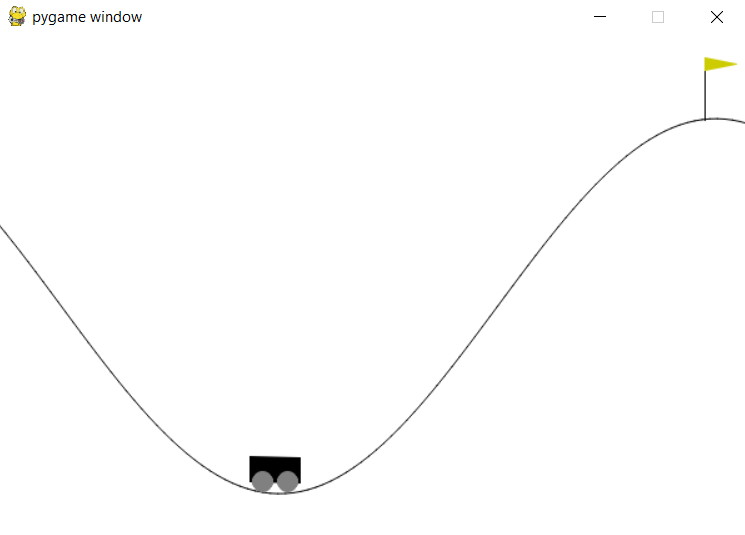
\includegraphics[width=10cm]{assets/mountain-car.png}}
    \caption{Rezultat pokretanja koda \ref{lst:init-code}}
    \label{fig:mountain-car}
\end{figure}

\subsection{Okolina}

Temelj oko kojeg se zasniva OpenAI Gym biblioteka jest razred \engl{class} \texttt{Env} koji u suštini implementira simulator koji pokreće okruženje u kojem naš agent može interaktirati s okolinom. Točnije rečeno, enkapsulira sva potrebna ponašanja i metode koje su potrebne za jednostavnu interakciju. Objekt tipa \texttt{Env} stvara se pozivanjem funkcije \texttt{gym.make()} (kod \ref{lst:init-code} linija 3) kojoj se predaje identifikator okoline (\texttt{id}) zajedno s opcionalnim argumentima (metapodatcima). 

\subsection{Interakcija s okolinom}

Kao što je vidljivo iz koda \ref{lst:init-code} osnovne metode koje se pozivaju nad instancom razreda \texttt{Env} su \texttt{reset} i \texttt{step}. Funkcija \texttt{reset} postavlja okruženje u početno stanje i vraća njegovu vrijednost (kod \ref{lst:init-code}. linija 5). S druge strane, funkciji \texttt{step} (kod \ref{lst:init-code}. linija 10) predaje se jedna od ispravnih akcija koja inicira prijelaz okoline iz jednog stanja u drugo. Funkcija vraća 4 vrijednosti: vrijednost prostora stanja \engl{observation}, iznos nagrade kao rezultat poduzimanja određene akcije  \engl{reward}, zastavicu koja signalizira jesmo li došli u završno stanje okoline \engl{done}, te neke dodatne informacije.

Još jedna vrlo često korištena funkcija jest \texttt{render} (kod \ref{lst:init-code}. linija 12) koja služi kako bi se u određenom formatu prikazala okolina. Dostupni formati su: \texttt{human} (otvara se skočni prozor sa slikom stanja okoline - slika \ref{fig:mountain-car}), \texttt{rgb_array} (\texttt{numpy} array RGB vrijednosti) i \texttt{ansi} (string reprezentacija okoline).

\subsection{Prostor akcija i prostor stanja}

Osnovna struktura okruženja opisana je atributima \texttt{observation_space} i \texttt{actio\-n_space} koji su dio razreda \texttt{Env} i čija se vrijednost može razlikovati zavisno o okolini. Atribut \texttt{action_space} opisuje numeričku strukturu svih legitimnih akcija koje se mogu izvesti nad određenom okolinom. S druge strane, atribut \texttt{observation_s\-pace} definira strukturu objekta koje predstavlja opis stanja u kojem se okolina nalazi.

Format validnih akcija i stanja okoline, odnosno struktura tih podataka, definirana je razredima \texttt{Box}, \texttt{Discrete}, \texttt{MultiBinary} i \texttt{MultiDiscrete}. Svi navedeni razredi nasljeđuju i implementiraju glavne metode nadrazreda \texttt{Space}. 

Razred \texttt{Box} predstavlja strukturu podataka u kontinuiranom $n$-dimenzionalnom prostoru. Prostor i njegove validne vrijednosti omeđene su gornjim i donjim granicama koje se jednostavno postave pri inicijalizaciji strukture pridruživanjem željenih vrijednosti atributima \texttt{high} i \texttt{low}. Kod \ref{lst:box-code} prikazuje inicijalizaciju \texttt{Box} strukture podataka koja je sastavljena od $3$-dimenzionalnog vektora čije su vrijednosti omeđene odozdo i odozgo vrijednostima $-1$ i $-2$. Metoda \texttt{sample(self)} nasumično uzorkuje element iz prostora koristeći različite distribucije ovisno o ograničenjima prostora.

\begin{listing}[H]
    \caption{Primjer korištenja strukture kontinuiranog prostora \texttt{Box}}
    \inputminted{python}{snippets/box.txt}
    \label{lst:box-code}
\end{listing}

Razred \texttt{Discrete} s druge strane, predstavlja strukturu podataka u diskretnom $n$-dimenzionalnom prostoru gdje su validne vrijednosti sve cjelobrojne vrijednosti unutar intervala $[0, n-1]$ (početna vrijednost se može specificirati). Kod \ref{lst:discrete-code} prikazuje inicijalizacije \texttt{Discrete} strukture podataka ovisno o specificiranoj početnoj vrijednosti.

\begin{listing}[H]
    \caption{Primjer korištenja strukture diskretnog prostora \texttt{Discrete}}
    \inputminted{python}{snippets/discrete.txt}
    \label{lst:discrete-code}
\end{listing}

\subsection{Omotači}

Omotači \engl{Wrappers} su prikladne strukture koje omogućavaju izmjenu elemenata postojećeg okruženja bez potrebe za mijenjanjem originalnog koda. Omotači omogućavaju modularnost, mogu se implementirati prema vlastitim potrebama i ulančavati. Ova funkcionalnost vrlo se često koristi u situacijama kada pri treniranju modela želimo normalizirati ulaze (skalirati piksele slike), provesti regularizaciju (podrezivanje vrijednosti nagrade), transformirati ulaze u Pytorch dimenzije, implementirati preskakanje slikovnih okvira...  Navedene funkcionalnosti moguće je postići tako da definiramo vlastiti omotač koji će nasljeđivati ili obični \texttt{Wrapper} nadrazred ili specifičnije razrede poput \texttt{ObservationWrapper}, \texttt{RewardWrapper}, \texttt{ActionWrapper}...

\subsection{Vektorizirana okruženja}

Koristeći standardne metode stvaranja i interakcije s Gym okruženjem, pokrećemo samo jednu instancu okruženja i na taj način ne iskorištavamo potpuno računalnu snagu koja nam je dostupna. Vektorizirana okruženja \engl{Vectorized environments} su okruženja koja paralelno pokreću više kopija istog okruženja u svrhu poboljšanja učinkovitosti i ubrzanja procesa učenja agenta.

?? TODO nastaviti ovo jer su sada objavili novu verziju u kojoj je već u Gym-u ukomponiran Vector API a ja sam do sada bio koristio njihov library \textit{baselines}. ?? - ponovna implementacija i usporedba

\begin{figure}[H]
    \centering
    \frame{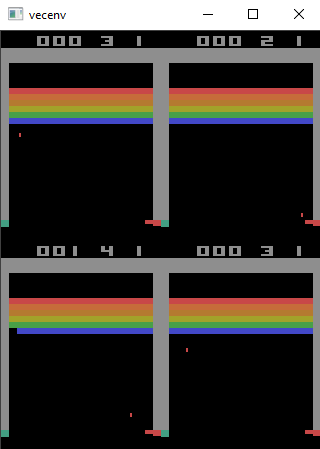
\includegraphics[height=9cm]{assets/breakout-vect.png}}
    \caption{Vektorizirano okruženje sa 4 paralelne asinkrone instance}
    \label{fig:breakout-vect}
\end{figure}

\section{Determinizam atari okruženja}

Upravljanje agentima i njihovo izvođenje akcija u određenoj atari okolini interno je implementirano koristeći objektno orijentiranu razvojnu cjelinu \engl{framework} \textit{The Arcade Learning Environment} (skraćeno \textit{ALE}). Na taj način razdvajaju se slojevi emulacije okruženja (koristeći Atari 2600 emulator \textit{Stella}), sloj koji kontrolira samog agenta \textit{(ALE)} i sloj koji pruža jednostavnu programsku implementaciju i interakciju \textit{(OpenAI Gym)} \cite{OpenAIALE}. 

Originalna Atari 2600 konzola nije imala izvor entropije za generiranje pseudoslučajnih brojeva i iz tog razloga okruženje je bilo u potpunosti determinističko - svaka igra počinje u istom stanju, a ishodi su u potpunosti određeni stanjem i akcijom \cite{AleDeterministic}. Iz tog razloga vrlo je jednostavno postići visoku uspješnost agenta u okolini pamćenjem dobrog niza akcija. Nama to ne odgovara jer želimo postići da agent nauči donositi dobre odluke. U novijim verzijama ALE-a i \textit{OpenAI Gym}-a implementirani su različiti pristupi za postizanje određenog stupnja stohastičnosti. 

Pristupi kojima se želi postići stohastičnost su ponavljanje prethodne akcije (engl. \textit{sticky actions}), nasumično preskakanje slikovnih okvira \engl{random frame skip}, odsustvo niza akcija na početku epizode \engl{initial no-ops} te postupak zamjene akcije drugom nasumično odabranom akcijom \engl{random action noise}. Navedeni pristupi mogu se specificirati prilikom instanciranja okoline. 

\section{Okruženja}

U OpenAI Gym ekosustavu dostupno je puno okruženja koja omogućuju interakciju s agentom. Neki od njih su: \textit{Atari} - skup od Atari 2600 okolina, \textit{MuJoCo} (punim nazivom \textit{Multi-Joint dynamics with Contact}) - skup okolina za provođenje istraživanja i razvoja u robotici, biomehanici, grafici i drugim područjima gdje je potrebna brzina i točna simulacija, \textit{Classic Control} - skup okolina koje opisuju poznate fizikalne eksperimente. Opisat ćemo neke od najkorištenijih okolina.

\subsection{Okruženje CartPole}

Ovo okruženje modelira fizikalni problem održavanja ravnoteže. Inačica je sličnog fizikalnog problema pod nazivom \textit{obrnuto njihalo} \engl{inverted pendulum}. Za pomična kolica zakvačen je stupić. Njegovo težište nalazi se iznad središta mase i na taj način osigurava da sustav nije stabilan.  Zglob, odnosno dodirna točka između stupića i kolica nema trenja niti drugih gubitaka. Također, kolica koja se kreću vodoravno po putanji u 2 smjera nemaju trenja niti drugih gubitaka. Cilj ovog fizikalnog problema jest uravnotežiti stup primjenom sila i pomicanjem kolica u lijevom ili desnom smjeru.

Za svaki poduzeti korak okolina dodjeljuje nagradu u vrijednosti $+1$. Struktura valjanih akcija koje agent može poduzeti (\texttt{action_space}) instanca je razreda \texttt{Disc\-rete(2)} - skup akcija je diskretan i u svakom koraku je moguće odabrati 1 od maksimalno 2 dostupne akcije. Opis značenja svake akcije prikazan je u tablici \ref{table:cart-pole-action}. S druge strane, objekt koji predstavlja strukturu stanja okoline u određenom vremenskom trenutku (\texttt{observation_space}) instanca je razreda \texttt{Box(4)} – stanje se sastoji od 4 kontinuirane vrijednosti od kojih su neke ograničene i odozdo i odozgo. Točan opis i granice vrijednosti predočeni su u tablici \ref{table:cart-pole-observation}.

\begin{table}[ht]
    \centering
    \caption{Opis valjanih akcija okoline CartPole - atribut \texttt{action_space}}
    \begin{tabular}{c c}
        \toprule
        Akcija & Opis akcije  \\
        \midrule
        0 & Pomak kolica ulijevo \\
        1 & Pomak kolica udesno \\
        \bottomrule
    \end{tabular}
    \label{table:cart-pole-action}
\end{table}

\begin{table}[ht]
    \centering
    \caption{Opis strukture okoline okoline CartPole - atribut \texttt{observation_space}}
    \begin{tabular}{c c c c}
        \toprule
        Indeks & Opis & Donja granica & Gornja granica \\
        \midrule
        0 & Pozicija kolica & $-4.8$ & $4.8$ \\
        1 & Brzina kolica & $-\infty$ & $\infty$ \\ 
        2 & Nagib štapića i kolica & $-0.418 \text{rad}$ & $0.418 \text{rad}$ \\
        3 & Brzina štapića na vrhu & $-\infty$ & $\infty$ \\
        \bottomrule
    \end{tabular}
    \label{table:cart-pole-observation}
\end{table}

Početno stanje okoline inicijalizira se pozivom metode \texttt{reset()} slučajnim vrijednostima iz uniformne razdiobe na intervalu $[- 0.05, 0.05]$. Okolina podržava 3 uvjeta zaustavljanja (uvjeti koji označuju da je riječ o terminalnom stanju): nagib štapića i kolica je izvan intervala $[-0.2095, 0.2095] \text{rad}$, pozicija sredine kolica je izvan intervala $[-2.4, 2.4]$ (sredina kolica dotiče rub vidljivog prostora) i duljina epizode veća je od $500$ koraka. Na slici \ref{fig:cart-pole} prikazana je okolina CartPole zajedno s vrijednostima okoline. % TODO napraviti svoje koje bolje izgleda

\begin{figure}[H]
    \centering
    \frame{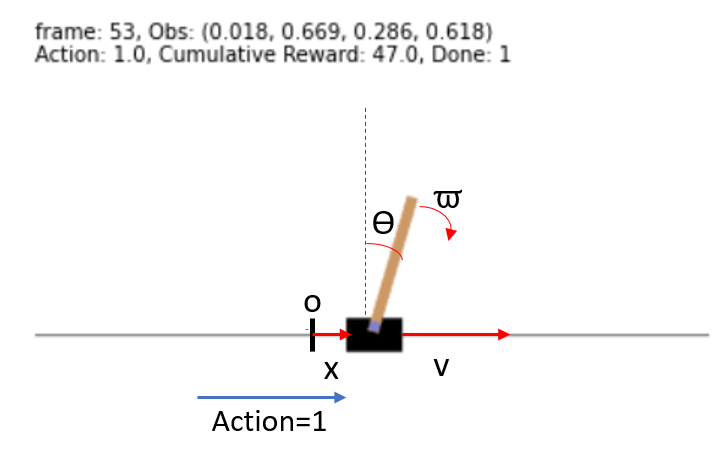
\includegraphics[height=5.5cm]{assets/cart-pole-not-mine.png}}
    \caption{Izgled i vrijednosti CartPole okoline - TODO}
    \label{fig:cart-pole}
\end{figure}

\subsection{Okruženje Breakout}

Ova okolina simulira poznatu Atari 2600 igru u kojoj je cilj sakupiti što više bodova pomičući platformu i održavajući lopticu na ekranu. Platforma je postavljena na dnu ekrana, na fiksnoj visini i moguće ju je pomicati u dva smjera. Loptica se odbija između zidova, platforme i 6 razina \textit{ciglenih} blokova čijim razbijanjem se sakupljaju bodovi. Ako loptica padne ispod platforme koju igrač kontrolira, gubi se život. Igra završava kada igrač potroši 5 života, odnosno kada 5 puta loptica padne ispod platforme. 

Skup validnih akcija je instanca razreda \texttt{Discrete(4)} - skup akcija je diskretan i u svakom koraku je moguće odabrati 1 od maksimalno 4 dostupne akcije. Opis značenja svake akcije prikazan je u tablici \ref{table:breakout-action}. Kao opis trenutnog stanja okoline moguće je dobiti RGB vrijednosti svakog piksela slike (slike dimenzije $210 \times 160$) ili vrijednosti radne memorije \textit{ALE} okoline (128 bajta) - što je korisno jer možemo preskočiti korak učenja reprezentacije okoline (preskačemo dio gdje algoritmi učenja moraju iz piksela slike naučiti reprezentaciju). Razlike u strukturi objekta okoline prikazane su u tablici \ref{table:breakout-observation}. 

\begin{table}[ht]
    \centering
    \caption{Opis valjanih akcija okoline Breakout - atribut \texttt{action_space}}
    \begin{tabular}{c c c}
        \toprule
        Akcija & Opis akcije & Detaljniji opis akcije  \\
        \midrule
        0 & NOOP & Ne poduzima se nikakva akcija \\
        1 & FIRE & Akcija koja pokreće igru \\ 
        2 & RIGHT & Platforma se pomiče udesno \\ 
        3 & LEFT & Platforma se pomiče ulijevo  \\
        \bottomrule
    \end{tabular}
    \label{table:breakout-action}
\end{table}

\begin{table}[H]
    \centering
    \caption{Opis strukture objekta okoline Breakout - atribut \texttt{observation_space}}
    \begin{tabular}{c c}
        \toprule
        Indeks & Struktura  \\
        \midrule
        RAM vrijednosti & \texttt{Box(0, 255, (128,), uint8)}  \\ 
        Vrijednosti RGB slike & \texttt{Box(0, 255, (210, 160, 3), uint8)}  \\
        \bottomrule
    \end{tabular}
    \label{table:breakout-observation}
\end{table}

Nagrada dolazi u obliku bodova koji se dobivaju uništavajući \textit{ciglene} blokove. Vrijednost nagrade ovisi o boji cigle. Izgled same okoline prikazan je na slici \ref{fig:breakout}.

\begin{figure}[H]
    \centering
    \frame{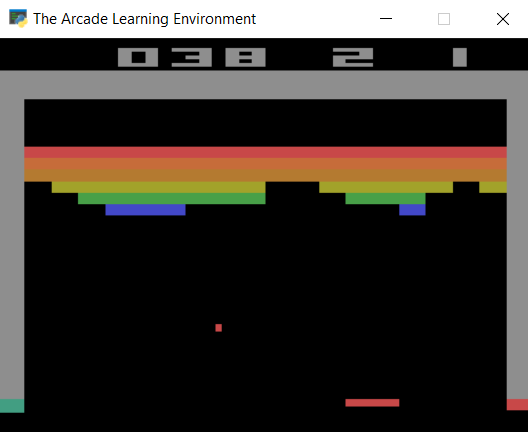
\includegraphics[width=10cm]{assets/breakout.png}}
    \caption{Okolina Breakout}
    \label{fig:breakout}
\end{figure}


% TODO dodati za literaturu https://blog.paperspace.com/getting-started-with-openai-gym/ i https://www.gymlibrary.ml/content/vector_api/ i https://www.gymlibrary.ml/ općenito

% TODO dodati za literaturu https://atariage.com/manual_html_page.php?SoftwareID=889

% značenje pojedinih ram pozicija https://github.com/mila-iqia/atari-representation-learning/blob/master/atariari/benchmark/ram_annotations.py

% https://stackoverflow.com/questions/45207569/how-to-interpret-the-observations-of-ram-environments-in-openai-gym
\chapter{Stable Baselines3}

Poznatije biblioteke otvorenog koda za programski jezik \textit{Python} koje prvenstveno pružaju implementacije algoritama podržanog učenja su \textit{Stable Baselines3}, \textit{RLlib}, \textit{Tensorforce}... Njihove implementacije algoritama i naučene modele korisno je koristiti pri usporedbi performansi vlastitih implementacija. Navedene biblioteke koriste \textit{OpenAI Gym} okruženja za razvijanje, testiranje i usporedbu agenata.

Stable Baselines3 (SB3) biblioteka sadrži skup implementacija algoritama podržanog učenja. Za oblikovanje dubokih modela korištena je \textit{PyTorch} biblioteka. Algoritmi su neovisni o modelu \engl{model-free} i ograničeni na interakciju jednog agenta s okolinom \engl{single-agent}. SB3 predstavlja nadogradnju \textit{Stable Baselines} i \textit{OpenAI Baselines} biblioteka koje za oblikovanje dubokih modela koriste \textit{TensorFlow} biblioteku. U odnosu na njih, SB3 je bolje dokumentiran, 95\% koda je pokriveno testovima \engl{test coverage}, te sadrži više implementiranih algoritama \cite{SB3}. 

Odsječak koda \ref{lst:sb3} prikazuje jednostavnost korištenja SB3 biblioteke. U dvije linije koda postavili smo tip dubokog modela, identifikator okoline, specificirali algoritam učenja, te pokrenuli učenje modela sa specificiranim ukupan broj koraka.

\begin{listing}[H]
    \caption{Jednostavan primjer korištenja \textit{Stable Baselines3} biblioteke}
    \inputminted{python}{snippets/sb3.py}
    \label{lst:sb3}
\end{listing}

\section{Korištenje predtreniranih modela}

Predtrenirane modele koji su objavljeni u javnom \textit{GitHub} repozitoriju \cite{sb3-alg-repo} koristit ćemo pri usporedbi ponašanja naših manualno implementiranih algoritama i pripadajućih agenata.

Za uspješno pokretanje agenata potrebno je proučiti javni \textit{GitHub} repozitorij radnog okvira \textit{RL Baselines3 Zoo} \cite{rl-zoo3}, klonirati projekt i pokrenuti naredbu \ref{lst:sb3-zoo} koja pokreće \textit{Python} skriptu s dodatnim argumentima u kojima je specificiran algoritam, identifikator okoline i direktorij u kojem se nalazi prednaučen agent. \textit{RL Baselines3 Zoo} jest radni okvir koji koristi \textit{Stable Baselines3} biblioteku i pruža niz korisnih skripti za treniranje i evaluiranje agenata, podešavanje hiperparametara, iscrtavanje rezultata i snimanje videa.

\begin{listing}[H]
    \caption{Naredba za izvođenje \textit{Python} skripte i pokretanje predtreniranog modela}
    \inputminted{powershell}{snippets/sb3-zoo.txt}
    \label{lst:sb3-zoo}
\end{listing}

\chapter{Implementacija}
\chapter{Moguća poboljšanja}

Korištenje drugih optimzacijskih postupaka osim Adam-a kao npr. SGD, SGD s momentom, SGD s restartom, RMSProp, RMSProp s momentom
Korištenje restarta kod promjene stope učenja... igranje s hiperparametrima

Implementacija ostalih algoritama podržanog učenja

Isprobati više verzija arhitekture dubokog modela i procijeniti benefite svakog.

Naučiti agente i provjeriti kako se ponašaju na novim vrstama okolina i kako se suočavaju s novim problemima.



\chapter{Zaključak}

U ovom radu proučena je i opisana problematika podržanog učenja gdje se bez znanja o pravilima i funkcioniranju specifične okoline, želi konstruirati agent kojemu je cilj pronaći optimalnu strategiju koja maksimizira očekivanu dobit u određenom vremenskom okviru. Agenti koji se prilično dobro ponašaju u takvim okolinama implementirani su pomoću različitih algoritama podržanog učenja koji se temelje na umjetnim neuronskim mrežama - jako dobrim univerzalnim aproksimatorima funkcija.

Proučeni su i opisani osnovniji modeli i ideje algoritama dubokog Q učenja, dvostrukog dubokog Q učenja, prednosnog akter-kritičara i popratnih inačica. Interakcijom i evaluacijom agenata koji su smješteni u posebnim okolinama, zapažene su prednosti i mane svakog od njih te su postignuti rezultati bliski onima \textit{state-of-the-art} algoritama i implementacija. 

Veliki broj algoritama, inačica, implementacija i dodataka čine podržano učenje izrazito velikim i iscrpnim područjem s velikim brojem primjena u stvarnom životu.

Podržano učenje duboko je inspirirano načinom kako ljudi i ostala živa bića uče iz iskustva pri interakciji s okolinom. Napretkom tehnologije, ideje umjetnih neuronskih mreža i algoritama, te razvitkom agenata koji u posebnim radnim okvirima interaktiraju s okolinom, sve smo bliži razvoju sustava opće umjetne inteligencije koje nije ograničeno na svoj strogi skup znanja koja mu definiraju samo jednu zadaću ili područje rada. Sve smo bliži tome da umjetna inteligencija bude inteligentna - sposobna učiti iz iskustva, prilagoditi se novim do sad neviđenim situacijama, razumjeti ih, iz konteksta učiti pravila koja definiraju ponašanje okoline te izvršavati zadatke i akcije koji su definirani tim pravilima na optimalan i posljedično koristan način.

\bibliography{literatura}
\bibliographystyle{fer}

\begin{sazetak}

Ovaj rad proučava problematiku podržanog učenja gdje se bez znanja o pravilima i funkcioniranju specifične okoline, želi konstruirati agent kojemu je cilj pronaći optimalnu strategiju koja maksimizira očekivanu dobit u određenom vremenskom okviru. Osim opisa podržanog učenja, dubokih modela i algoritama koji se baziraju na dubokim modelima, detaljno je prezentirana struktura \textit{OpenAI Gym} biblioteke i njenih okolina, te napravljena usporedba u kojoj se analizira uspješnost naučenih agenata dubokog Q učenja, dvostrukog dubokog Q učenja te prednosnog akter-kritičara.

Programsko rješenje implementirano je u programskom jeziku \textit{Python}, primarno koristeći \textit{PyTorch} radni okvir za dizajn i učenje dubokih neuronskih mreža, te \textit{OpenAI Gym} biblioteka za simulaciju i testiranje ponašanja agenata.

\kljucnerijeci{Podržano učenje, duboko učenje, OpenAI Gym, algoritmi neovisni o modelu, duboko Q učenje, dvostruko duboko Q učenje, prednosni akter-kritičar}
\end{sazetak}

\engtitle{Automated design of agents for various environments}
\begin{abstract}

This paper studies the issue of reinforcement learning where without knowing the rules and internal dynamics of environment, the goal is to build an agent whose aim is to find the optimal strategy that maximizes the expected reward in a given time frame. Aside from describing the basics of reinforcement learning, deep learning models and model free algorithms, the key concepts of \textit{OpenAI Gym} library and its environments are broken down in detail, and a comparison is made between agents implemented using Deep Q Networks, Double Deep Q Networks and Advantage Actor Critic Networks.

Software implementation is written in \textit{Python}, primarily using the \textit{PyTorch} framework for designing and learning deep neural networks, and the \textit{OpenAI Gym} library for simulating and testing agent behavior.

\keywords{Reinforcement learning, deep learning, OpenAI Gym, model-free algorithms, Deep Q Networks, Double Deep Q Networks and Advantage Actor Critic}
\end{abstract}


\listoffigures
\listoftables

\clearpage
\renewcommand\listoflistingscaption{Popis programskih isječaka}
\addcontentsline{toc}{chapter}{\listoflistingscaption}
\listoflistings

\end{document}
